\documentclass[../../../../main.tex]{subfiles}
\begin{document}

\begin{flushright}
\footnotesize\textit{【自動文字起こし・要確認】}
\end{flushright}

\noindent
[\textbf{解}] (イ) 判別式 $D$ として
\begin{align*}
D &= (a+c)^2 - 4(ac-b^2) \\
&= 4b^2 + (a-c)^2 \ge 0
\end{align*}
より、与方程式は実根を持つ。 \quad \text{同}

\vspace{0.5cm}

\noindent
(ロ)
\[
\begin{cases}
\alpha + \beta = a + c \\
\alpha \beta = ac - b^2
\end{cases}
\]
\[
\gamma - \alpha = \frac{a+c}{2} - \alpha - \frac{(a-c)(p^2-q^2)+4bpq}{2(p^2+q^2)}
\]
この正負は、以下とひとしい
\begin{align*}
A &= (a+c)(p^2+q^2) - 2\alpha(p^2+q^2) - (a-c)(p^2-q^2) - 4bpq \\
&= 2cp^2 + 2aq^2 - 2\alpha(p^2+q^2) - 4bpq
\end{align*}
\[
\frac{A}{2} = (c-\alpha)p^2 - 2bpq + (a-\alpha)q^2 \equiv f(p)
\]
$c = \alpha$ つまり $b=0$ の時、$f(p) = (a-\alpha)q^2 \ge 0$ となって $\gamma \ge \alpha$ である。 $c > \alpha$ の時、$f(p)=0$ の判別式 $D'$ として
\[
D'/4 = [b^2 - (c-\alpha)(a-\alpha)]q^2 = 0
\]
より、グラフの形を考えて $f(p) \ge 0 \iff \gamma \ge \alpha$。よっていずれの場合も $\gamma \ge \alpha \dots$ ①が成り立つ

\[
\beta - \gamma = \beta - \frac{a+c}{2} + \frac{(a-c)(p^2-q^2)+4bpq}{2(p^2+q^2)}
\]
この正負は、以下とひとしい
\begin{align*}
B &= 2\beta(p^2+q^2) - (a+c)(p^2+q^2) + (a-c)(p^2-q^2) + 4bpq \\
&= 2\beta(p^2+q^2) - 2aq^2 - 2cp^2 + 4bpq
\end{align*}
\[
\frac{B}{2} = (\beta-c)p^2 + 2bpq + (\beta-a)q^2 \equiv g(p)
\]
$\beta = c$ つまり $b=0$ のとき、$g(p) = (\beta-a)q^2 \ge 0$ から $\beta \ge \gamma$。 $\beta > c$ の時、同様に判別式 $D''$ として
\[
D''/4 = [b^2 - (\beta-c)(\beta-a)]q^2 = 0
\]
だから、$\beta \ge \gamma$。以上より $\beta \ge \gamma$ も成立つ $\dots$ ②

\noindent
①, ②から常に $\alpha \le \gamma \le \beta$ が成立する \quad \text{同}

\begin{center}
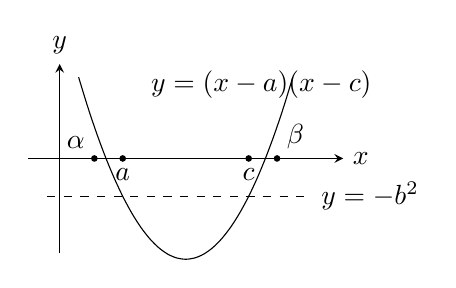
\begin{tikzpicture}[scale=0.8, >=stealth]
  \draw[->] (-0.5,0) -- (4.5,0) node[right] {$x$};
  \draw[->] (0,-1.5) -- (0,1.5) node[above] {$y$};
  \draw[domain=0.3:3.7, smooth, variable=\x] plot ({\x}, {(\x-1)*(\x-3)-0.6});
  \node[above] at (3.2,0.8) {$y=(x-a)(x-c)$};
  \draw[dashed] (-0.2,-0.6) -- (4.0,-0.6) node[right] {$y=-b^2$};
  \fill (0.55, 0) circle (1.5pt) node[above left] {$\alpha$};
  \fill (1, 0) circle (1.5pt) node[below] {$a$};
  \fill (3, 0) circle (1.5pt) node[below] {$c$};
  \fill (3.45, 0) circle (1.5pt) node[above right] {$\beta$};
\end{tikzpicture}
\end{center}
\noindent
※ 以上の証明に、$\alpha \le a, c \le \beta$ を用いたが、これはグラフより明らかである（対称性から $a \le c$ とした）

\newpage

\end{document}
